\chapter{Fundamentação Teórica}
Este capitulo busca contextualizar os principais conceitos abordados no presente trabalho, tais como os materiais utilizados como base e também a tecnologia adotada no desenvolvimento do projeto. E ao final, serão elencados alguns trabalhos correlatos.

\section{ENEF}
A Estratégia Nacional de Educação Financeira (ENEF) representa uma resposta proativa e estruturada às crescentes demandas de uma sociedade que enfrenta desafios financeiros complexos. Instituída com o claro objetivo de aprimorar a conscientização financeira da população brasileira, a ENEF busca não apenas promover a cidadania, mas também equipar os indivíduos com as ferramentas necessárias para tomar decisões financeiras informadas.

Esta estratégia abrange um amplo espectro de áreas de estudo, que vão desde os direitos e deveres básicos até tópicos mais complexos, como investimentos, previdência e planejamento financeiro. A inclusão de temas como poupança, crédito, seguros e consumo demonstra a abordagem abrangente adotada pela ENEF. Ao abordar temas tão variados, a ENEF reconhece e enfatiza que a educação financeira é um processo contínuo, que deve começar na infância e continuar ao longo da vida.

\subsection{Material Didático}
A ENEF destaca-se por sua abordagem prática, evidenciada por sua ampla variedade de materiais didáticos. Foram elaborados 24 livros especificamente alinhados com a missão educacional da ENEF. Cada livro foi cuidadosamente desenvolvido para atender às necessidades de diferentes faixas etárias: 18 destinados ao Ensino Fundamental e os 6 restantes focados no Ensino Médio. Uma característica notável é a separação dos livros em materiais específicos para alunos e guias para professores, garantindo que o conteúdo seja adequadamente direcionado para cada público.

Os primeiros livros têm como objetivo familiarizar os alunos do Ensino Fundamental com conceitos fundamentais de cidadania. Através de situações cotidianas, como a organização de uma sala de aula ou a coordenação de eventos escolares, os alunos são introduzidos a princípios de planejamento e organização. Conforme avançam na série, são gradualmente expostos a temas financeiros mais sofisticados, desde o entendimento básico das contas domésticas até a compreensão da origem e da trajetória do dinheiro na sociedade.

Dentre os materiais didáticos, os livros-jogo se destacam por suas narrativas envolventes. Ao invés de simplesmente transmitir informações, esses livros contam histórias que permitem aos alunos explorar cenários financeiros e entender as consequências de várias decisões. Esse enfoque narrativo é enriquecido por discussões em livros subsequentes, que oferecem insights sobre o papel de diferentes instituições financeiras e seu impacto na sociedade.

Nos 5º e 6º livros da série ENEF, observa-se uma abordagem pedagógica inovadora e envolvente, que reflete a excelência e o comprometimento da ENEF em proporcionar uma educação financeira de qualidade. Estes volumes adotam um formato interativo chamado "livro-jogo". Enquanto o jogo digital foca na jogabilidade, o livro-jogo se destaca por sua capacidade de envolver o leitor em uma narrativa rica, permitindo-lhe tomar decisões que influenciam os rumos da história.

A Figura 1 ilustra um esquema que destaca alguns dos caminhos possíveis que a história pode seguir. Este diagrama demonstra a complexidade e a diversidade de trajetórias que um jogador pode experimentar, refletindo diferentes escolhas financeiras e suas respectivas consequências.

\begin{figure}[ht]
	\centering
	\caption{Esquema com alguns dos caminhos possíveis da primeiro jogo/história.}
	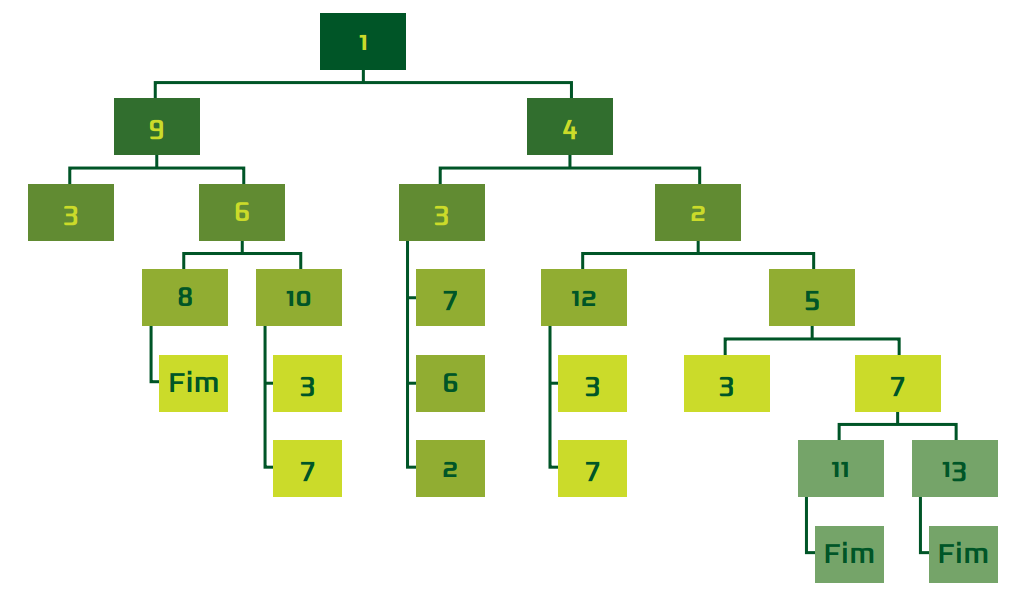
\includegraphics[scale=0.3]{Textuais/Pictures/Picture1.png}
	\fonte{\cite{Educacao_financeira_nas_escolas_professor}}\label{fig:figure-1}
\end{figure}

As Figuras 2 e 3 retratam momentos cruciais na narrativa do livro-jogo. Em cada figura, o leitor é introduzido a um cenário e, posteriormente, confrontado com duas ou três opções de ação. Cada escolha desencadeia diferentes desenvolvimentos na história, ilustrando as implicações de suas decisões no mundo financeiro.

\begin{figure}[ht]
	\centering
	\caption{Momento de decisão com duas possibilidades de caminhos.}
	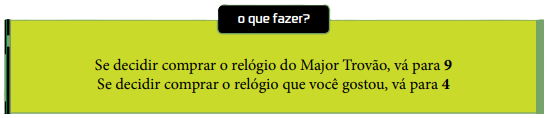
\includegraphics[scale=1]{Textuais/Pictures/Picture2.png}
	\fonte{\cite{Educacao_financeira_nas_escolas}}\label{fig:figure-2}
\end{figure}
\begin{figure}[ht]
	\centering
	\caption{Momento de decisão com duas possibilidades de caminhos.}
	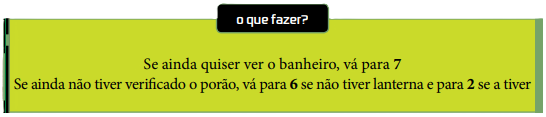
\includegraphics[scale=1]{Textuais/Pictures/Picture3.png}
	\fonte{\cite{Educacao_financeira_nas_escolas}}\label{fig:figure-3}
\end{figure}

\newpage

Na continuação da série, principalmente nas fases finais do Ensino Fundamental, a ENEF aprofunda a abordagem, introduzindo conceitos mais avançados e específicos sobre o universo financeiro. Os alunos são expostos a uma variedade de instituições financeiras e suas respectivas funções. Por exemplo, ao aprender sobre bancos, os estudantes ganham insights sobre operações bancárias, sistemas de crédito e a importância da gestão financeira. Quando o tema é agências de viagens ou hotéis, os alunos são introduzidos ao mundo das transações comerciais, tarifas, reservas e a economia do turismo. Essa abordagem detalhada serve para ampliar o horizonte dos alunos e prepará-los para interações financeiras mais complexas no futuro.

\section{RPG Maker MZ}
O RPG Maker MZ é uma plataforma robusta de desenvolvimento de jogos, especializada em jogos de interpretação de personagens (RPG). Esta ferramenta oferece uma ampla gama de recursos pré-construídos e interfaces intuitivas, possibilitando que desenvolvedores, possam criar experiências interativas ricas e complexas. \cite{RPGMakerMZ}

\begin{figure}[ht]
	\centering
	\caption{Interface do RPG Maker MZ.}
	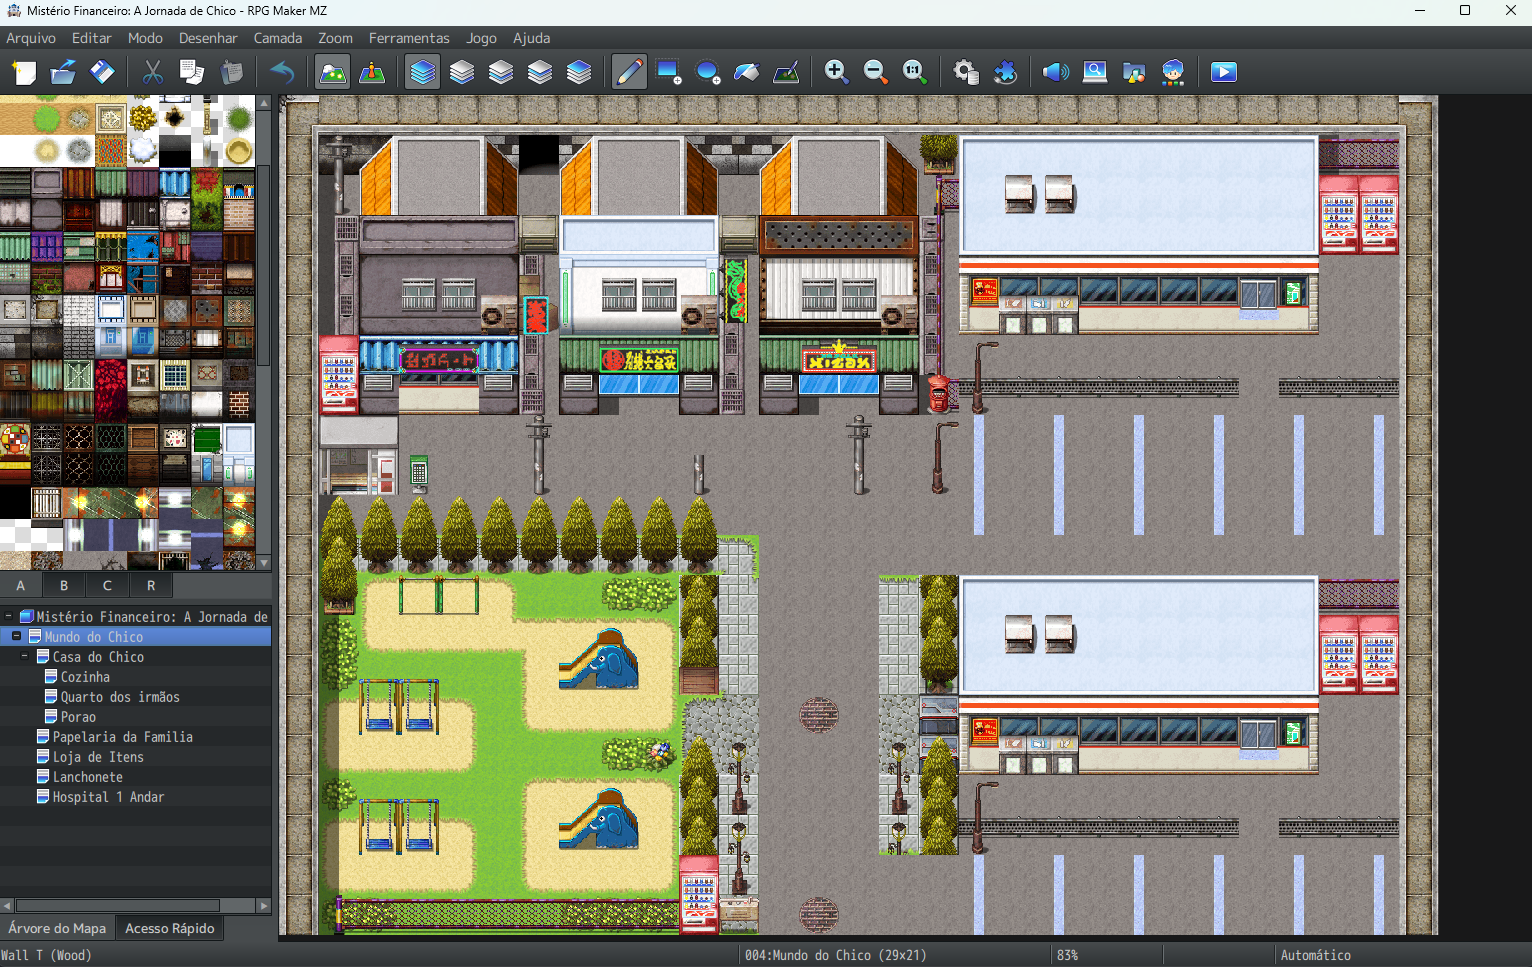
\includegraphics[scale=0.3]{Textuais/Pictures/RPGMaker_Interface.png}
	\fonte{Captura de tela do autor (2023).}\label{fig:rpgmaker-interface}
\end{figure}

\subsection{Recursos e Funcionalidades}
O RPG Maker MZ oferece uma série de recursos que facilitam a criação de um ambiente educacional interativo. Entre eles estão:

\begin{itemize}
	\item \textbf{Comandos de Evento:} Interface para criação de eventos que inclui exibição de texto, escolhas, controle de variáveis, e mais, facilitando a construção narrativa e interações no jogo.

	      \begin{figure}[ht]
		      \centering
		      \caption{Comandos disponíveis na página 1 do event commands do RPG Maker MZ.}
		      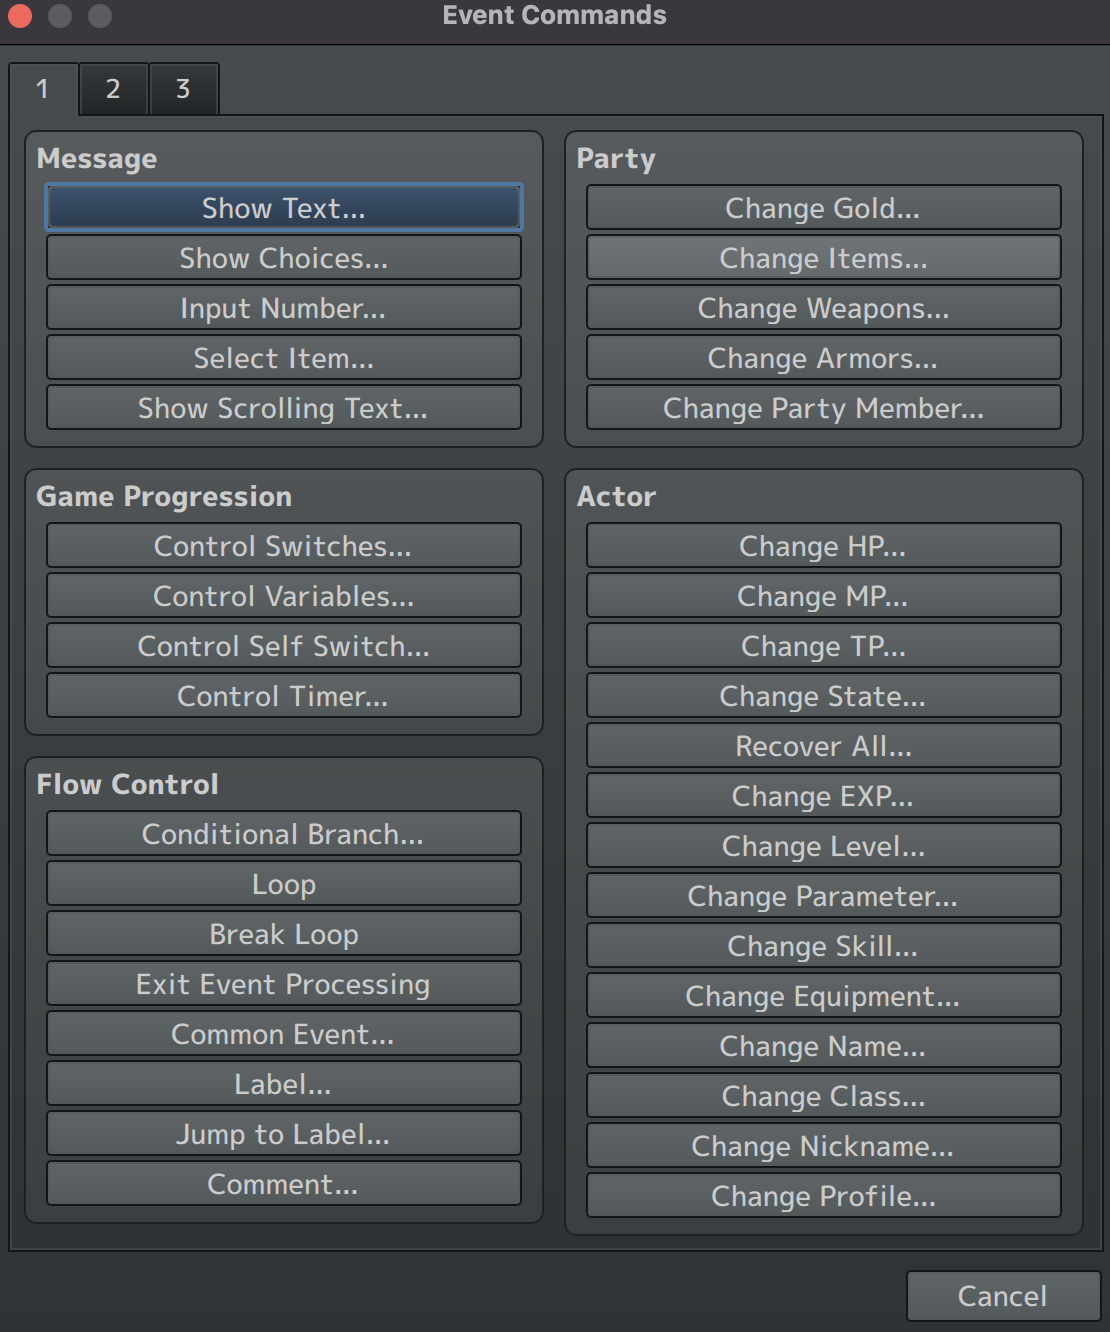
\includegraphics[scale=0.3]{Textuais/Pictures/Event-commands-1.png}
		      \fonte{Captura de tela do autor (2023).}\label{fig:rpgmaker-event-commands-1}
	      \end{figure}

	      \begin{figure}[ht]
		      \centering
		      \caption{Comandos disponíveis na página 2 do event commands do RPG Maker MZ.}
		      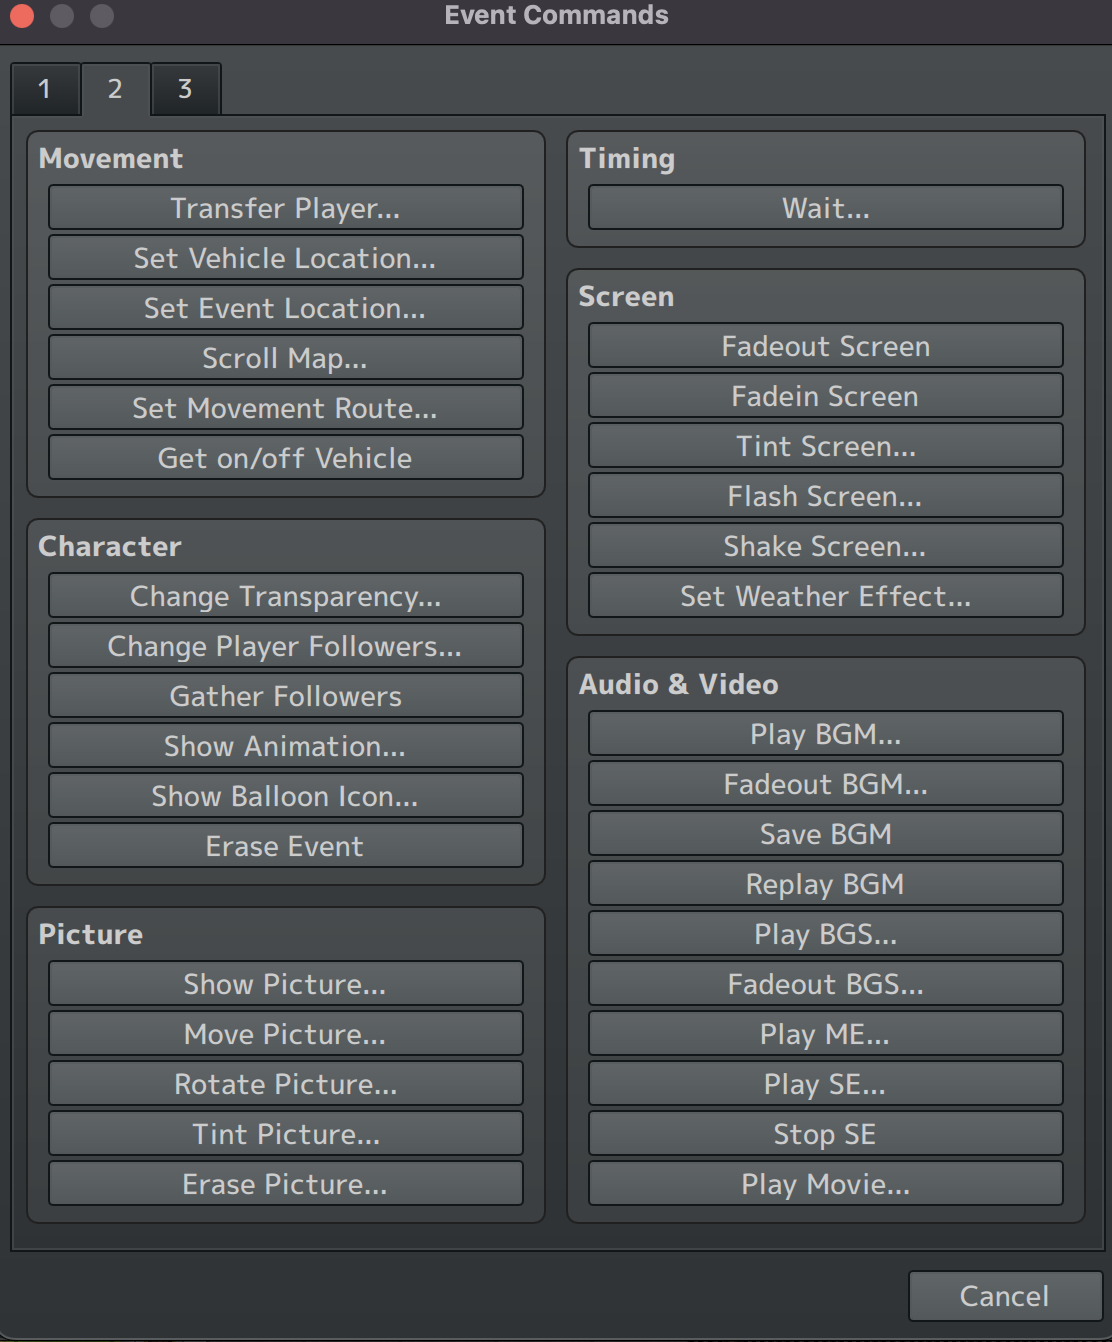
\includegraphics[scale=0.3]{Textuais/Pictures/Event-commands-2.png}
		      \fonte{Captura de tela do autor (2023).}\label{fig:rpgmaker-event-commands-2}
	      \end{figure}

	      \begin{figure}[ht]
		      \centering
		      \caption{Comandos disponíveis na página 3 do event commands do RPG Maker MZ.}
		      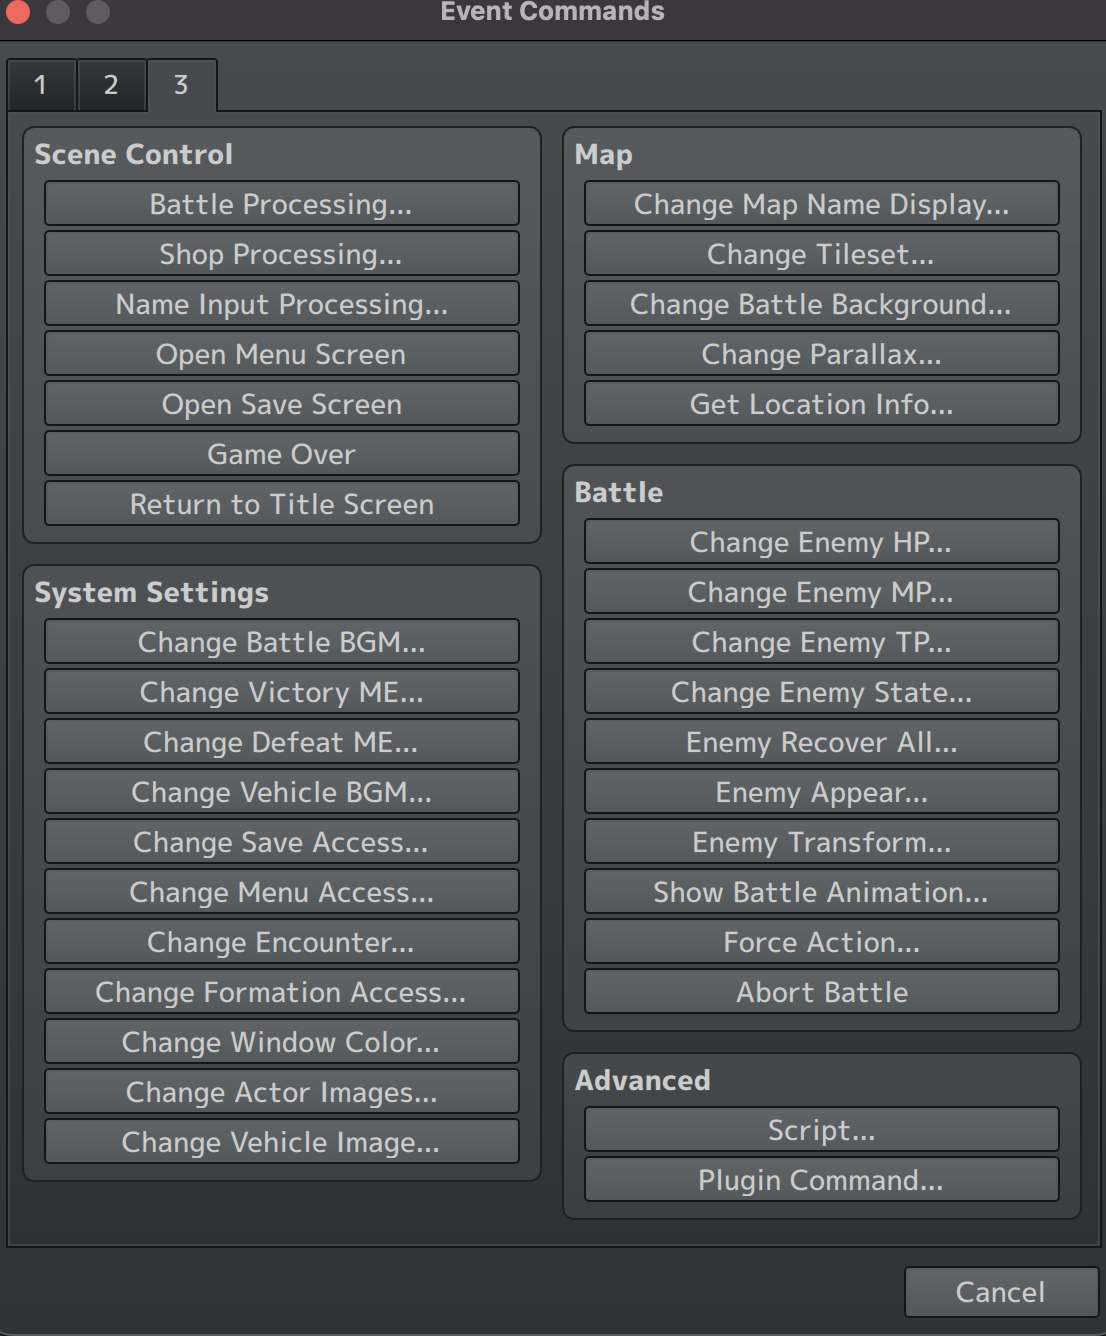
\includegraphics[scale=0.3]{Textuais/Pictures/Event-commands-3.png}
		      \fonte{Captura de tela do autor (2023).}\label{fig:rpgmaker-event-commands-3}
	      \end{figure}

	      \newpage

	\item \textbf{Criador de Personagens:} Oferece um conjunto de ferramentas para a criação de personagens personalizados. Os usuários podem selecionar entre uma variedade de faces, cabelos, expressões, roupas e acessórios, permitindo uma personalização detalhada dos avatares do jogo.

	      \begin{figure}[ht]
		      \centering
		      \caption{Interface de criação de personagens do RPG Maker MZ.}
		      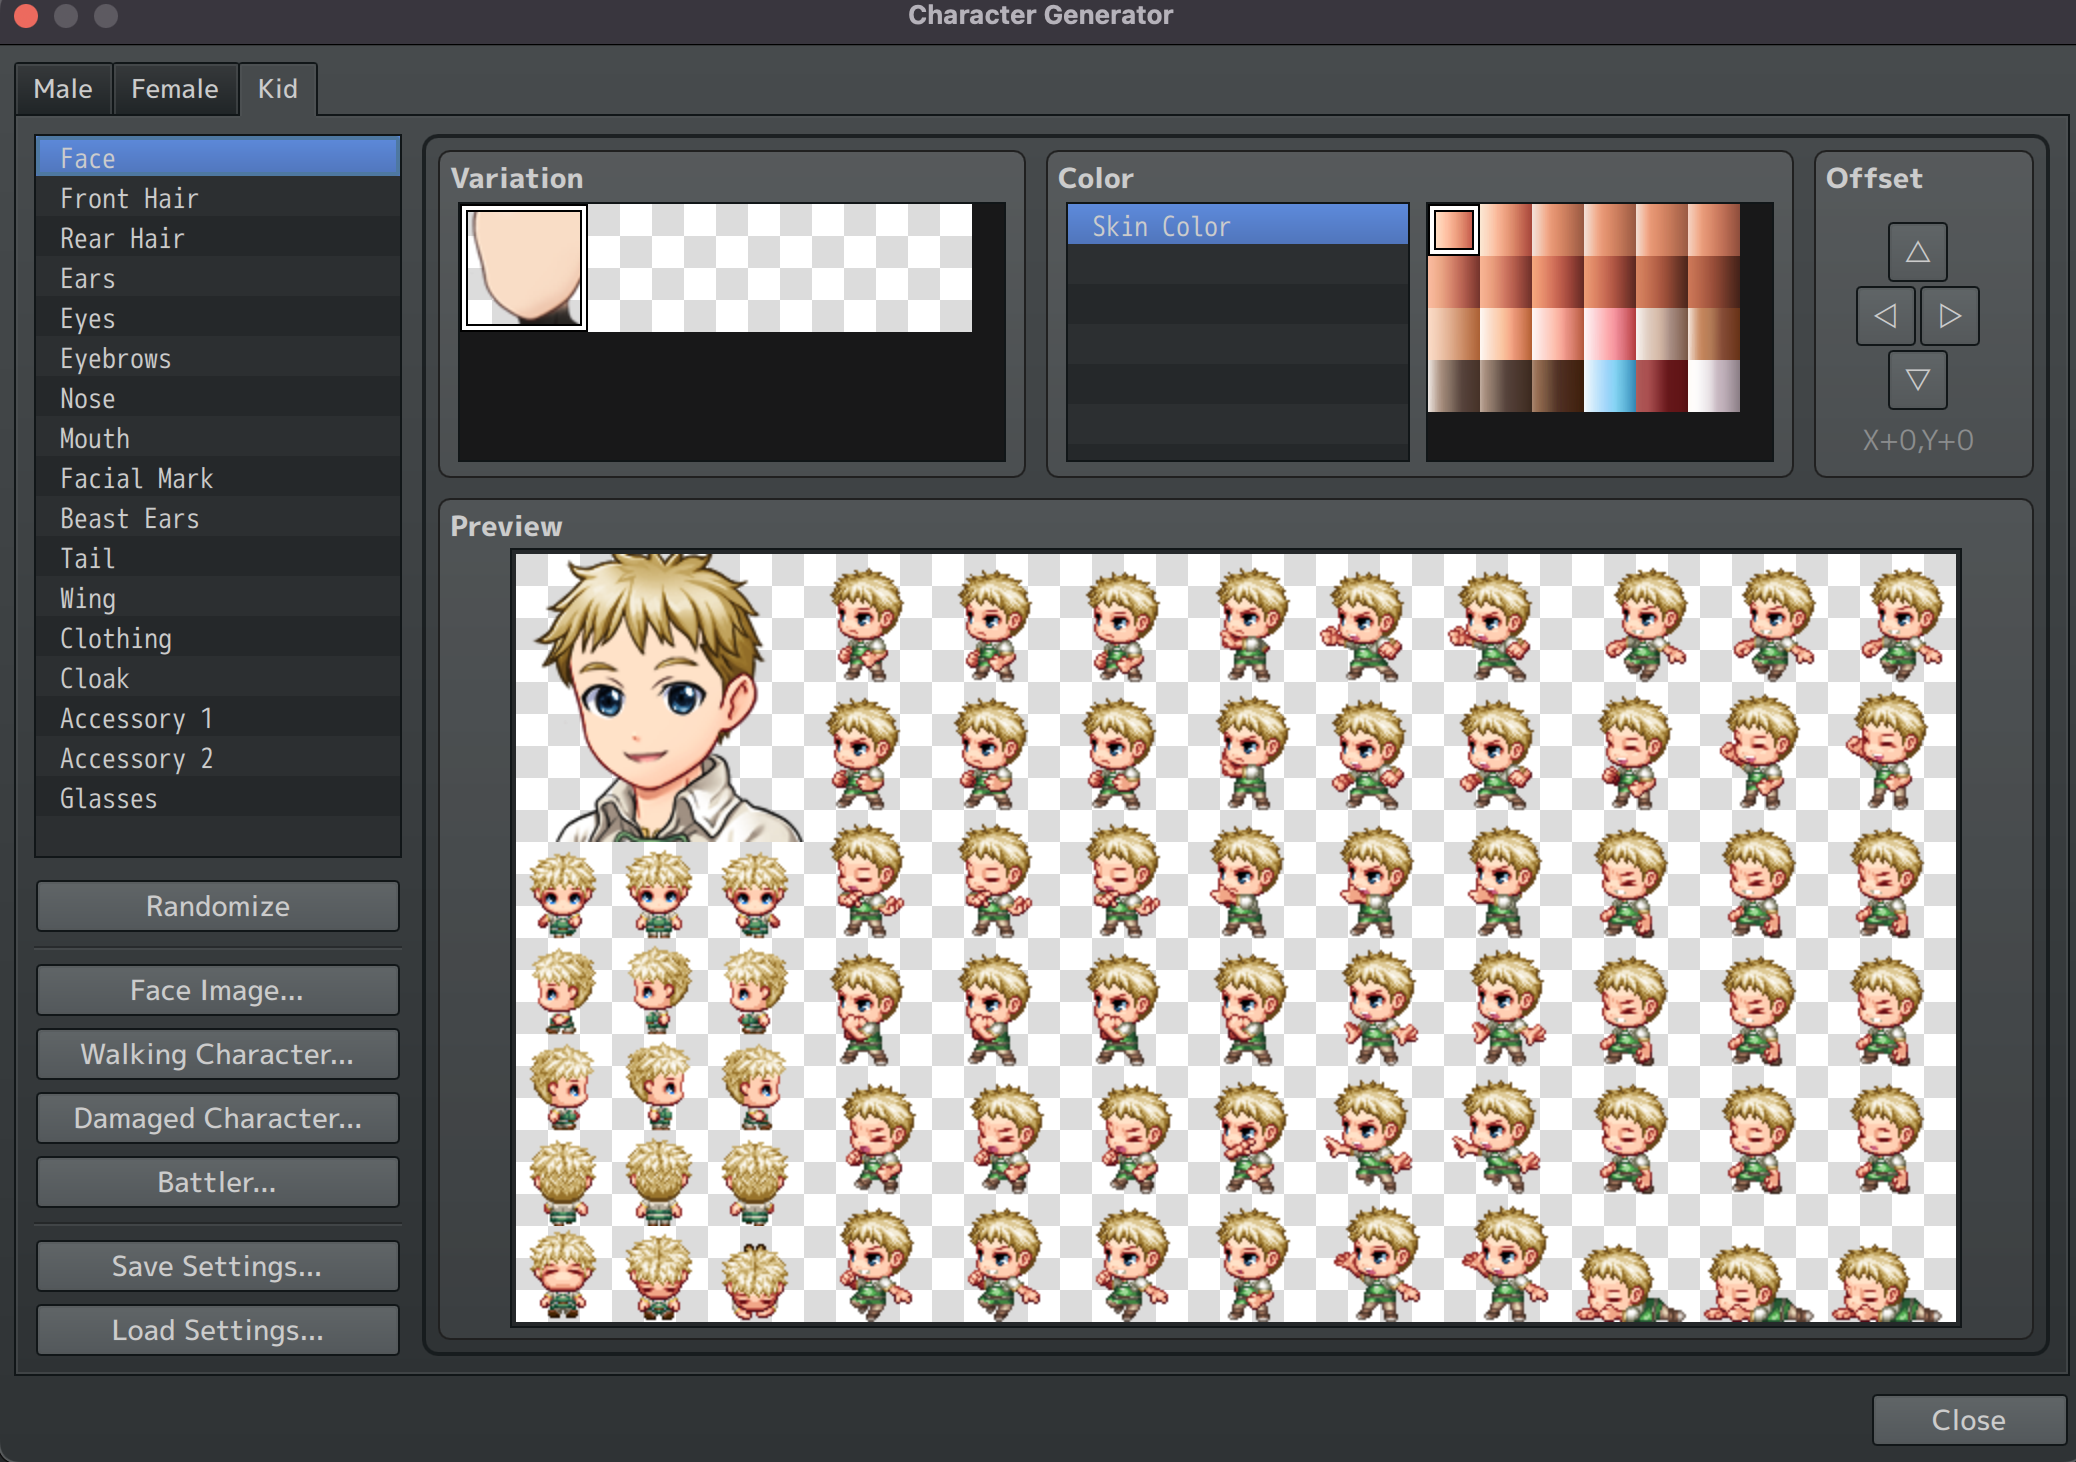
\includegraphics[scale=0.3]{Textuais/Pictures/Picture5.png}
		      \fonte{Captura de tela do autor (2023).}\label{fig:rpgmaker-criador-personagens}
	      \end{figure}

	\item \textbf{Banco de Dados:} Disponibiliza um banco de dados abrangente para o gerenciamento de elementos do jogo como itens, habilidades e inimigos, essencial para a criação de uma jogabilidade rica e envolvente.

	      \begin{figure}[ht]
		      \centering
		      \caption{Interface do Banco de Dados do jogo no RPG Maker MZ.}
		      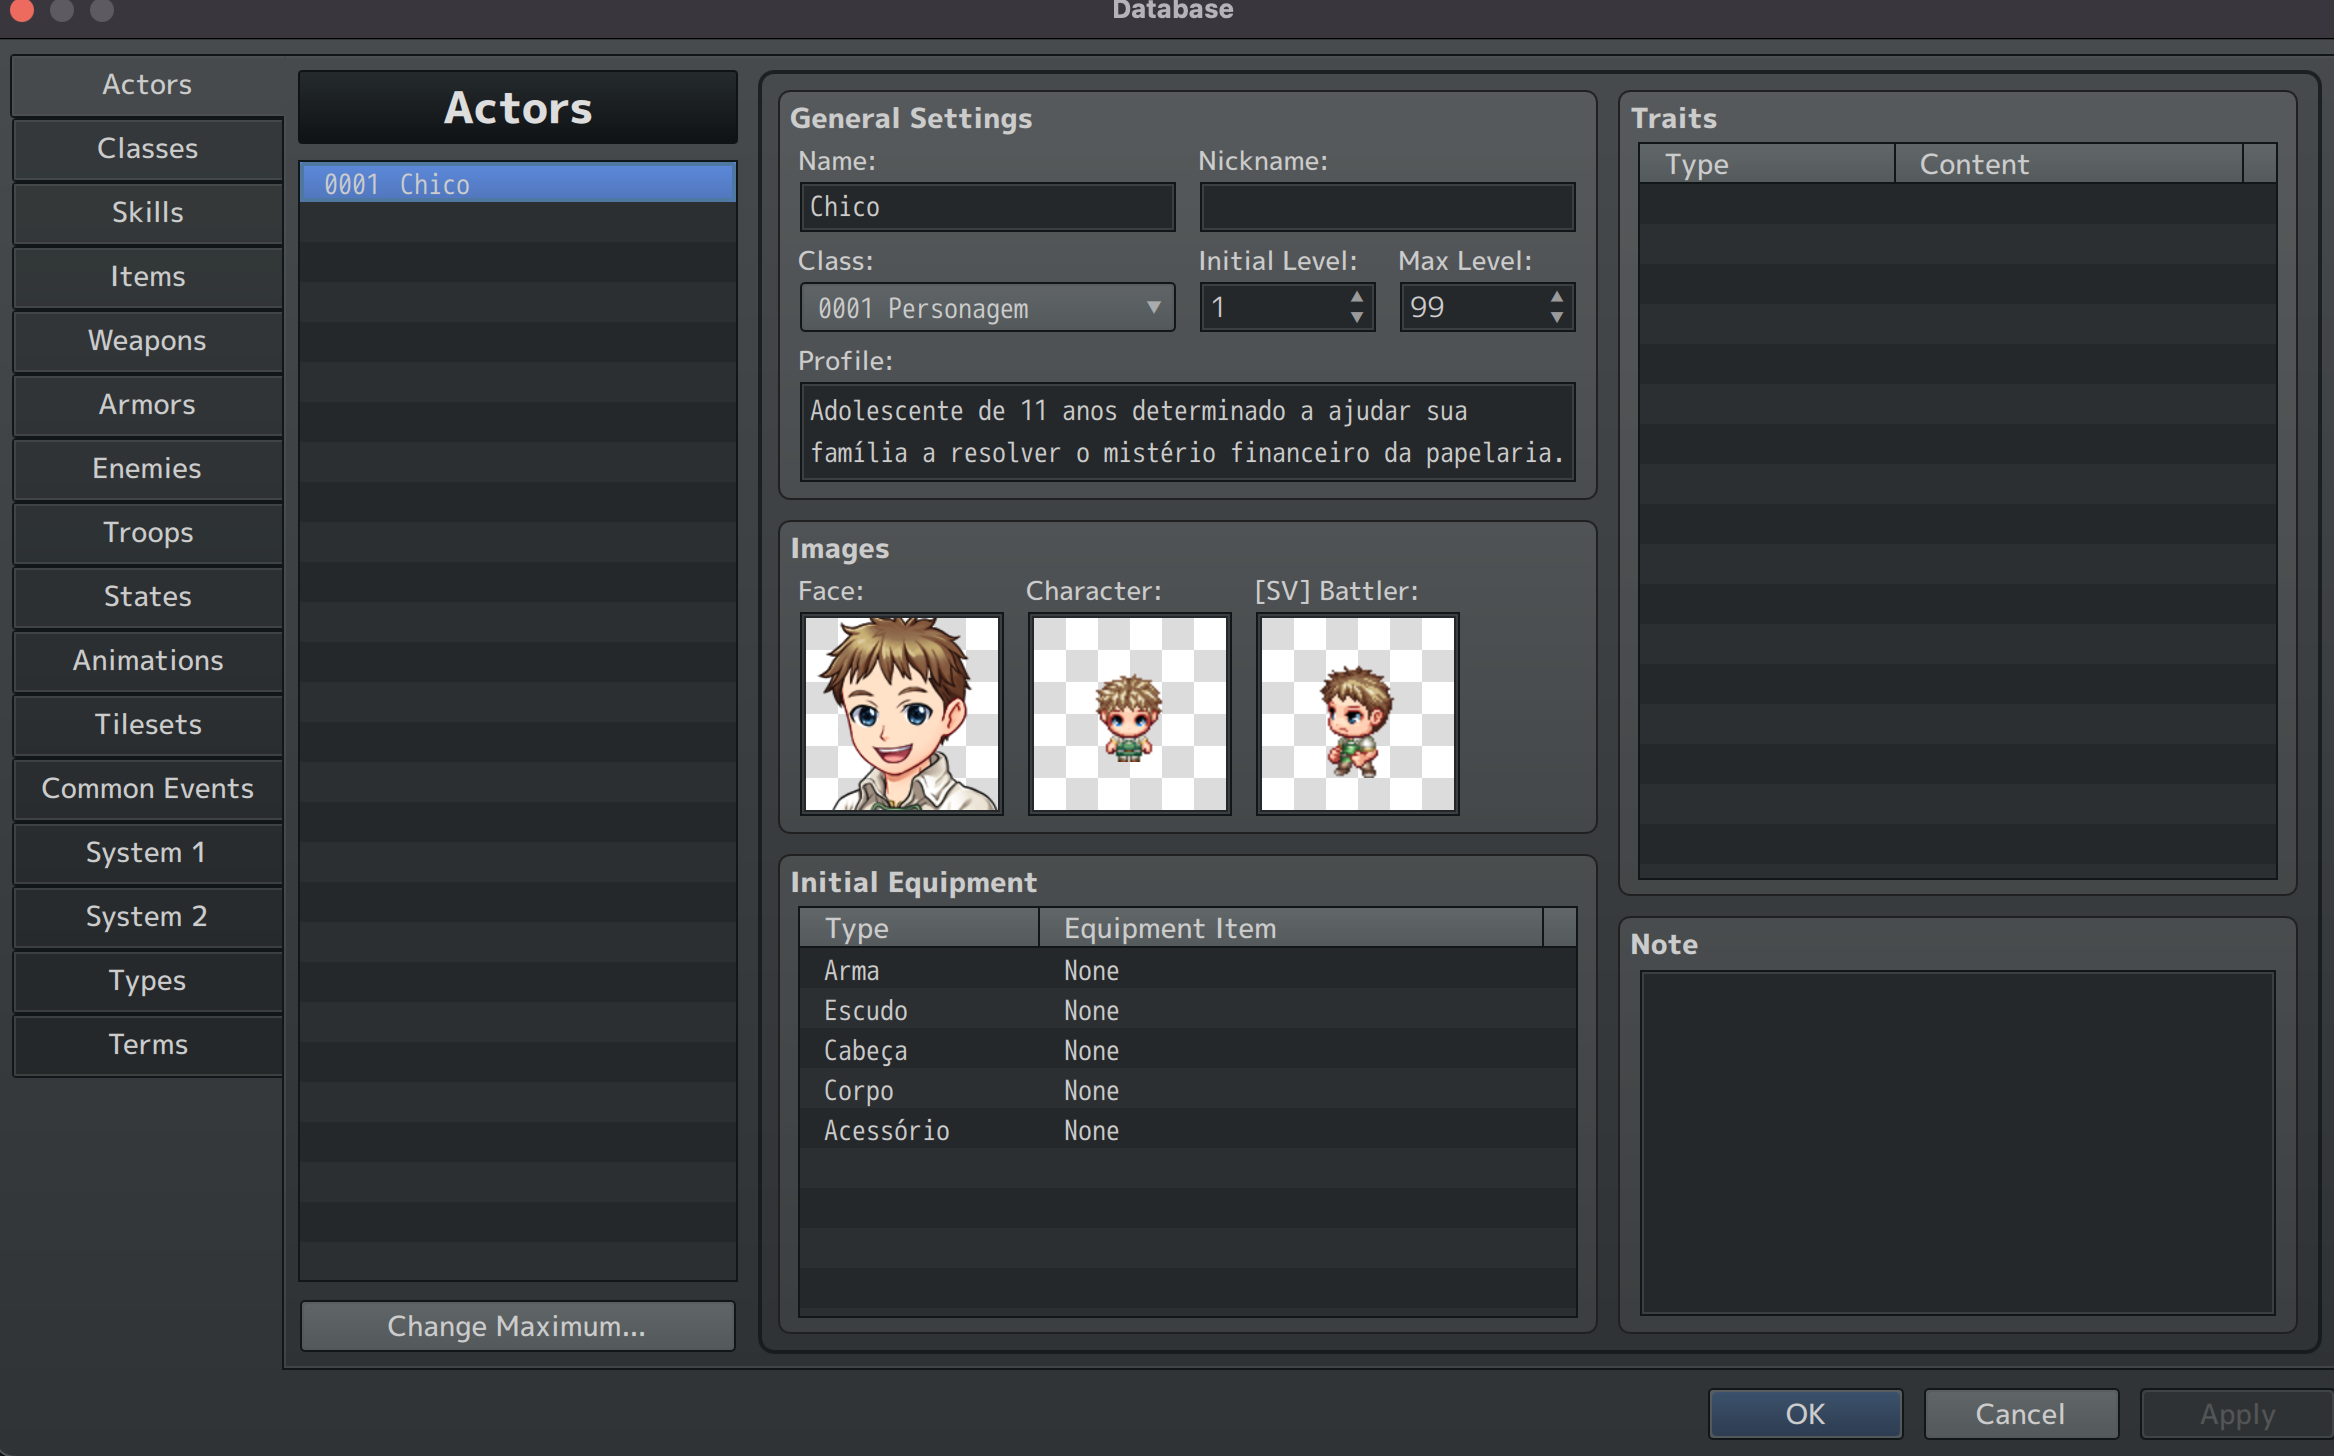
\includegraphics[scale=0.3]{Textuais/Pictures/DataBase.png}
		      \fonte{Captura de tela do autor (2023).}\label{fig:rpgmaker-interface-database}
	      \end{figure}


	      \newpage

	\item \textbf{Tilesets:} Disponibiliza uma vasta coleção de tilesets, que são conjuntos de imagens utilizadas para construir os mapas do jogo, permitindo a criação de mundos detalhados e variados.

	      \begin{figure}[ht]
		      \centering
		      \caption{Interface de gestão de Tilesets do RPG Maker MZ.}
		      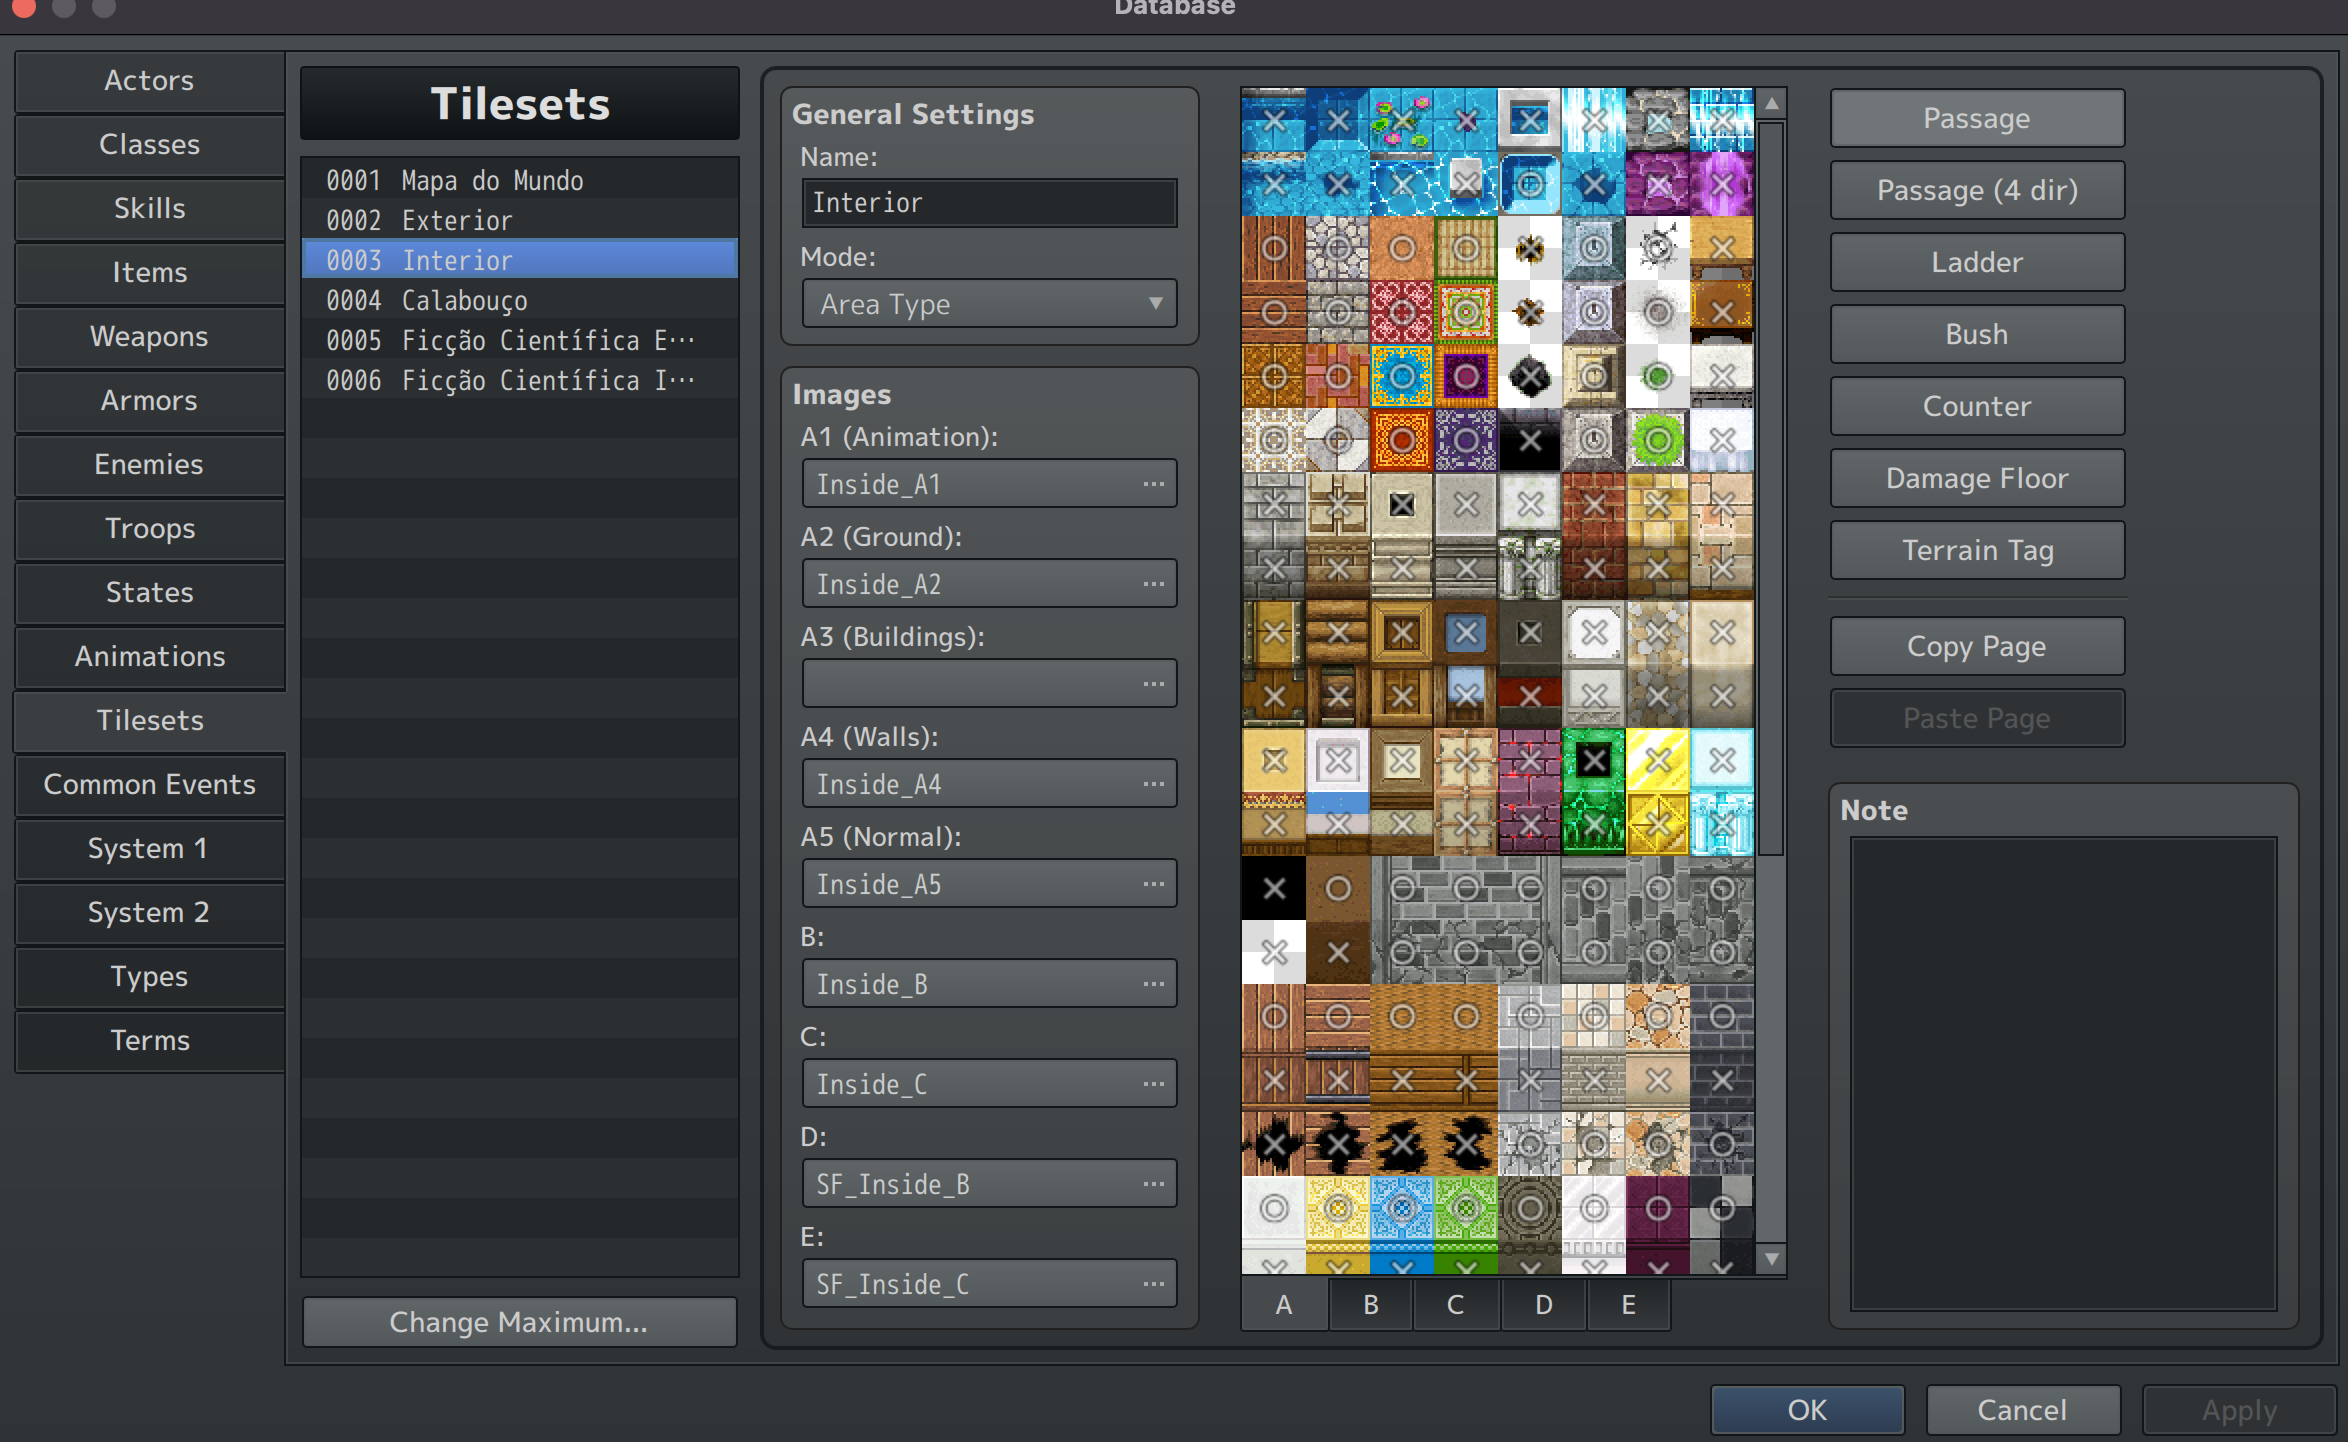
\includegraphics[scale=0.3]{Textuais/Pictures/Tileset.png}
		      \fonte{Captura de tela do autor (2023).}\label{fig:rpgmaker-interface-tilesets}
	      \end{figure}

\end{itemize}

\section{GIMP}

O GIMP (GNU Image Manipulation Program) é uma ferramenta de edição de imagens de código aberto, robusta e multiplataforma, que se revela uma escolha eficiente para a edição de TileSets utilizados no RPG Maker MZ. Sua funcionalidade de manipulação de imagens permite aos desenvolvedores modificar e criar TileSets personalizados, proporcionando um nível adicional de personalização e originalidade aos mapas do jogo. O GIMP suporta uma ampla gama de formatos de arquivo e oferece um leque de ferramentas de edição, desde simples cortes e ajustes de cores até operações complexas de manipulação de camadas e efeitos. \cite{GIMP_Documentation}

\begin{figure}[ht]
	\centering
	\caption{Interface de Edição de imagem do GIMP.}
	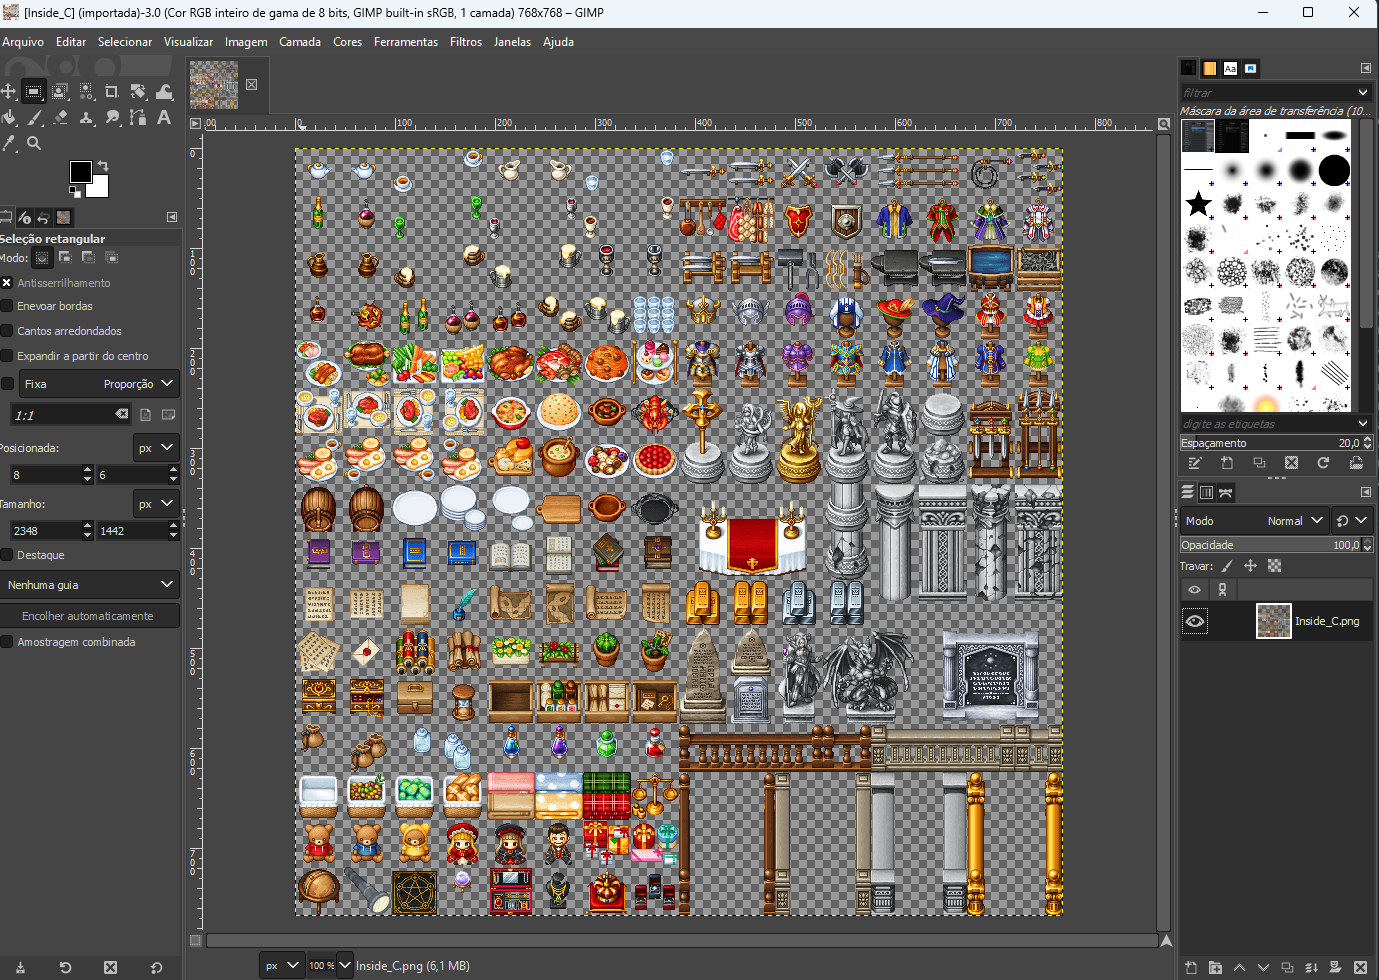
\includegraphics[scale=0.4]{Textuais/Pictures/Gimp.png}
	\fonte{Captura de tela do autor (2023).}\label{fig:gimp-interface}
\end{figure}


\section{Trabalhos Correlatos}
Nesta seção, apresentam-se trabalhos que, de alguma forma, se correlacionam com o presente estudo, oferecendo uma perspectiva sobre as diversas abordagens em jogos educativos focados na educação financeira.

\subsection{Debt Maze}
O \textit{Debt Maze} \cite{Debt_Maze} representa um marco na integração de conceitos financeiros em jogos digitais. Este jogo utiliza um labirinto repleto de desafios baseados em temas financeiros, como empréstimos, juros e pagamentos em atraso, para criar uma experiência envolvente que adapta-se a jogadores de diferentes níveis de conhecimento em finanças. A mecânica de navegação pelo labirinto simboliza as decisões financeiras na vida real, integrando elementos imersivos e persuasivos para educar e entreter o jogador. Esta abordagem lúdica contribui significativamente para a alfabetização financeira, incentivando decisões mais informadas.

Comparativamente, o presente trabalho distingue-se do \textit{Debt Maze} por adotar uma abordagem prática e cotidiana, mais adequada ao público infantil. Ao invés de um jogo de labirinto, propõe-se cenários reais e ferramentas interativas para simular decisões financeiras, aproximando o aprendizado à realidade das crianças.

\begin{figure}[ht]
	\centering
	\caption{Interface do Debt Maze.}
	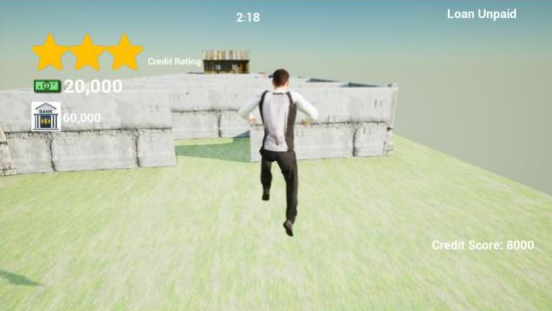
\includegraphics[scale=0.9]{Textuais/Pictures/debt-maze-1.png}
	\fonte{\textit{Debt Maze} \cite{Debt_Maze}.}\label{fig:debt-maze-1}
\end{figure}

\begin{figure}[ht]
	\centering
	\caption{Interface do Debt Maze.}
	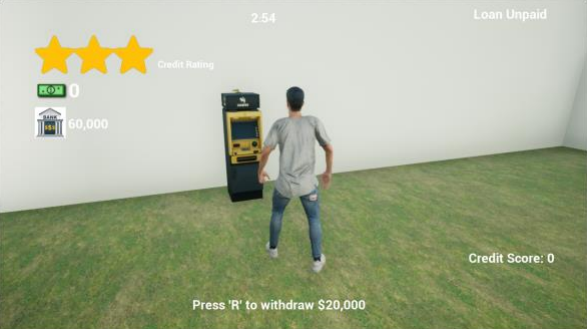
\includegraphics[scale=0.8]{Textuais/Pictures/debt-maze-2.png}
	\fonte{\textit{Debt Maze} \cite{Debt_Maze}.}\label{fig:debt-maze-2}
\end{figure}

\subsection{PlanCash}
O \textit{PlanCash} \cite{mariano2020educaccao}, um inovador jogo de tabuleiro, combina educação e entretenimento, utilizando a estrutura lúdica para ensinar matemática e gestão financeira a um público infantil. Este jogo aborda conceitos como a história do dinheiro e economia por meio de um tabuleiro interativo, onde os jogadores enfrentam situações-problema que estimulam a reflexão e análise financeira. Esta abordagem didática destaca-se por integrar o aprendizado financeiro em atividades cotidianas, oferecendo uma base sólida para o entendimento infantil de conceitos financeiros e matemáticos.

Em contraste, o presente trabalho avança esta ideia com uma proposta digital, atraente à geração atual de crianças, combinando elementos visuais e interativos para enriquecer a experiência educacional, alinhando o aprendizado financeiro às tecnologias contemporâneas.

\begin{figure}[ht]
	\centering
	\caption{Manual do \textit{PlanCash}.}
	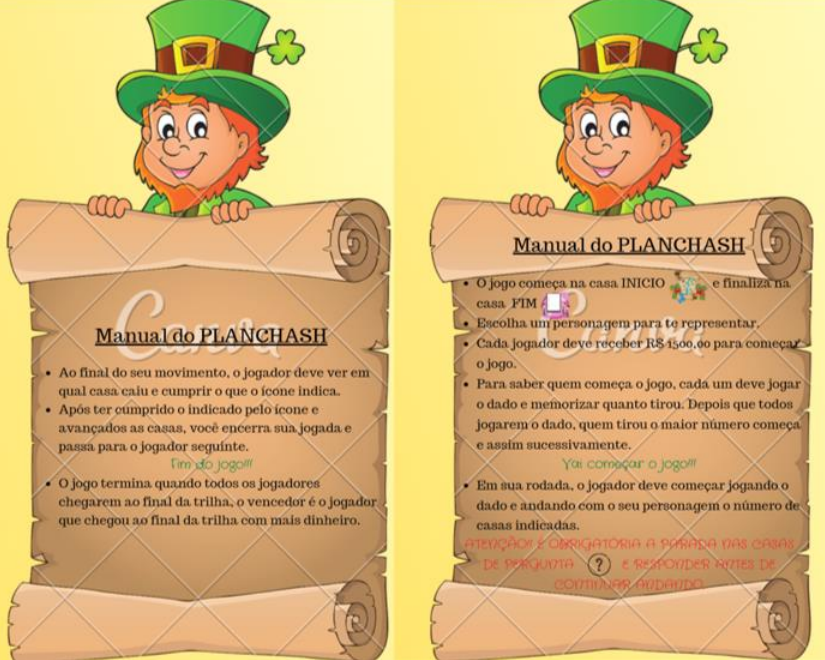
\includegraphics[scale=0.5]{Textuais/Pictures/Plancash-1.png}
	\fonte{\textit{PlanCash} \cite{mariano2020educaccao}.}\label{fig:plancash-1}
\end{figure}

\begin{figure}[ht]
	\centering
	\caption{Tabuleiro do \textit{PlanCash}.}
	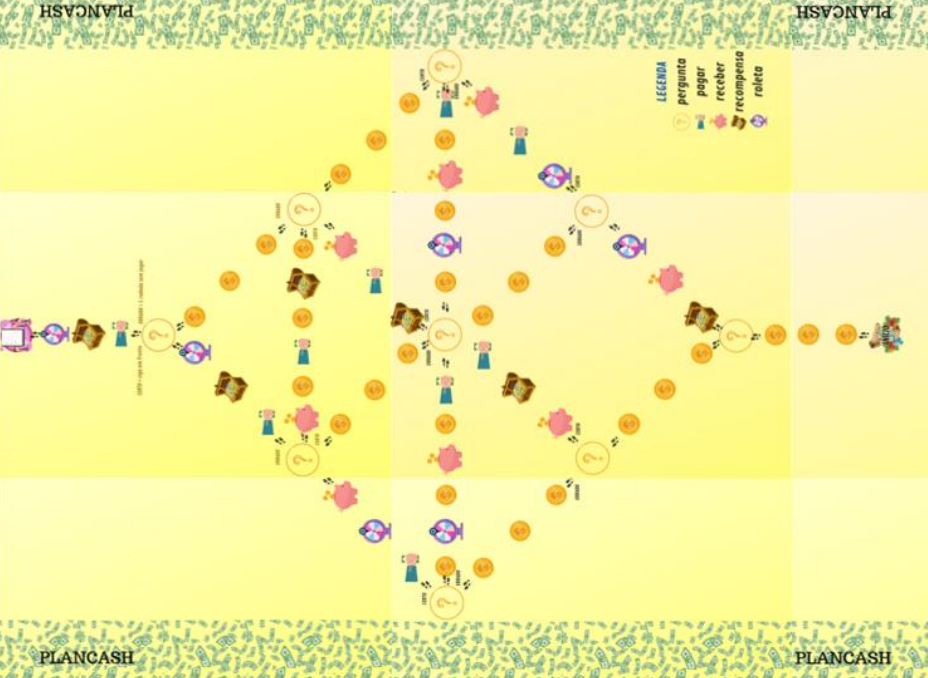
\includegraphics[scale=0.5]{Textuais/Pictures/Plancash-2.png}
	\fonte{\textit{PlanCash} \cite{mariano2020educaccao}.}\label{fig:plancash-2}
\end{figure}

\newpage

\subsection{Finance Game}
O \textit{Finance Game} \cite{Finance_Game} adota uma abordagem de simulação para a educação financeira, oferecendo aos jogadores cenários da vida adulta, como a gestão de um orçamento pessoal. Este jogo destaca-se por seu foco na tomada de decisões financeiras equilibradas, promovendo um entendimento prático sobre responsabilidade financeira e bem-estar pessoal. A interação com elementos simulados do cotidiano, como mercado e banco, proporciona aos jogadores uma vivência educacional que transcende a mera teoria, enfatizando a importância de escolhas conscientes.

O presente trabalho, em comparação, foca em uma imersão mais alinhada à realidade infantil, oferecendo cenários e decisões financeiras que se conectam diretamente às experiências e compreensão das crianças, facilitando a assimilação dos conceitos de educação financeira.

\begin{figure}[ht]
	\centering
	\caption{Tela Inicial do \textit{Finance Game}.}
	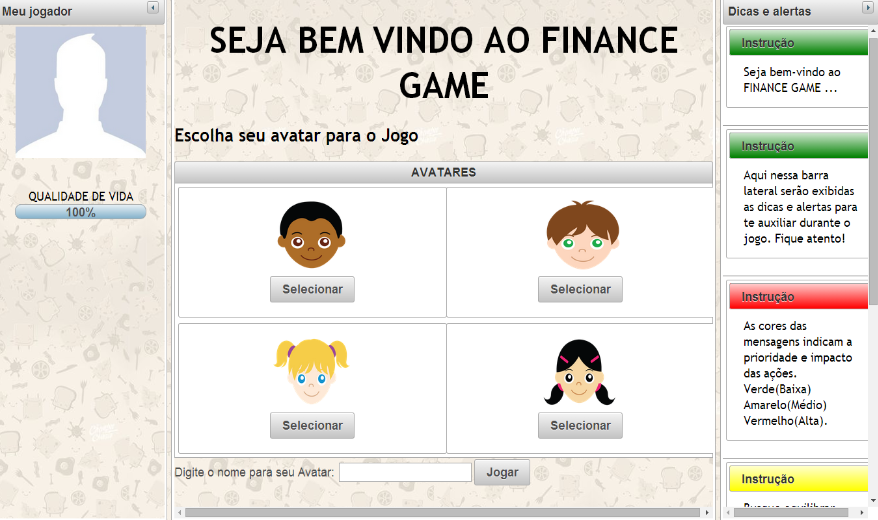
\includegraphics[scale=0.6]{Textuais/Pictures/Finance-game-1.png}
	\fonte{\textit{Finance Game} \cite{Finance_Game}.}\label{fig:finance-game-1}
\end{figure}

\begin{figure}[ht]
	\centering
	\caption{Cena do Mercado em \textit{Finance Game}.}
	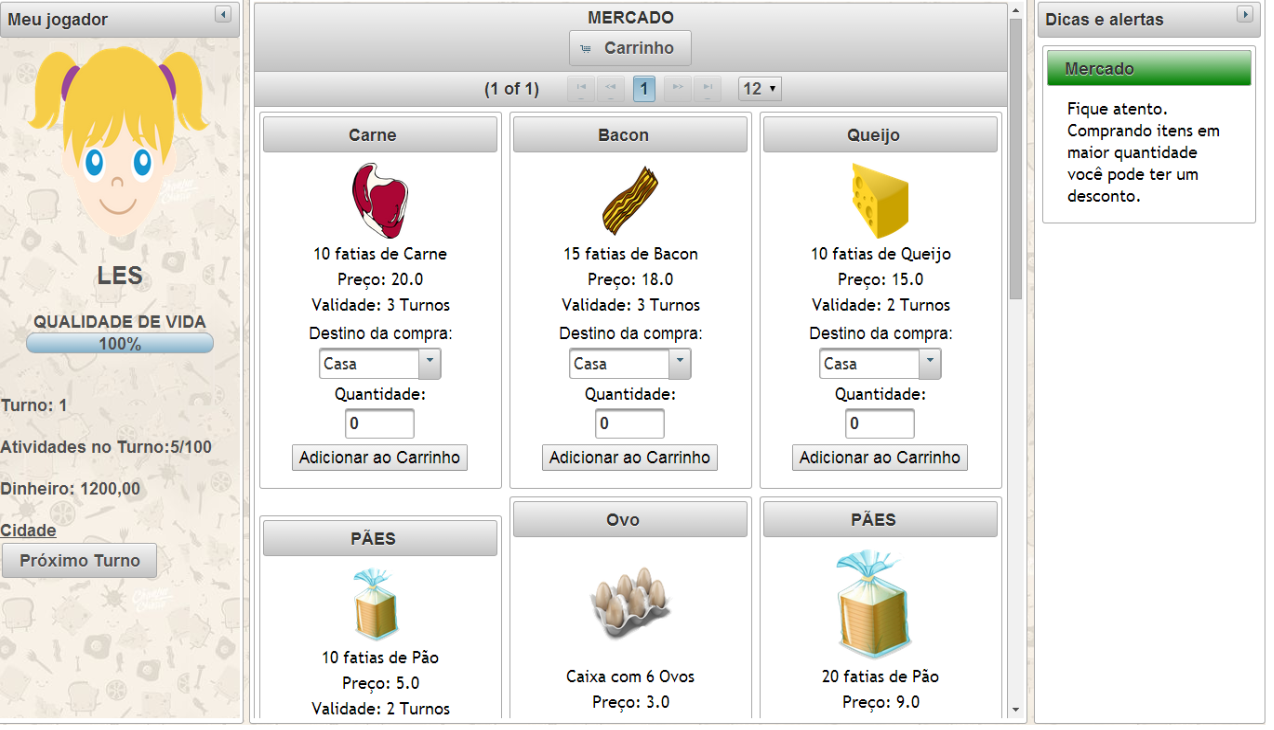
\includegraphics[scale=0.4]{Textuais/Pictures/Finance-game-2.png}
	\fonte{\textit{Finance Game} \cite{Finance_Game}.}\label{fig:finance-game-2}
\end{figure}

\newpage

\subsection{InvestPlay}
O \textit{InvestPlay} \cite{santos2020investplay} é um exemplo de jogo educativo que combina diversão e aprendizado em finanças. Este jogo introduz os jogadores à gestão de ativos e passivos, utilizando uma mecânica interativa de perguntas e respostas. O nível desafiador de algumas perguntas é uma consideração importante, especialmente para o público infantil. A personalização do jogo para diferentes temas educativos é um ponto forte, permitindo adaptar o conteúdo ao nível de compreensão das crianças.

Comparando-o com o presente estudo, busca-se refinar a proposta educacional do \textit{InvestPlay}, alinhando os conteúdos especificamente ao entendimento infantil. Esta abordagem simplificada visa tornar os conceitos financeiros mais acessíveis e relevantes para crianças, facilitando a assimilação eficaz dos princípios financeiros.

\begin{figure}[ht]
	\centering
	\caption{Tela de instruções iniciais do \textit{InvestPlay}.}
	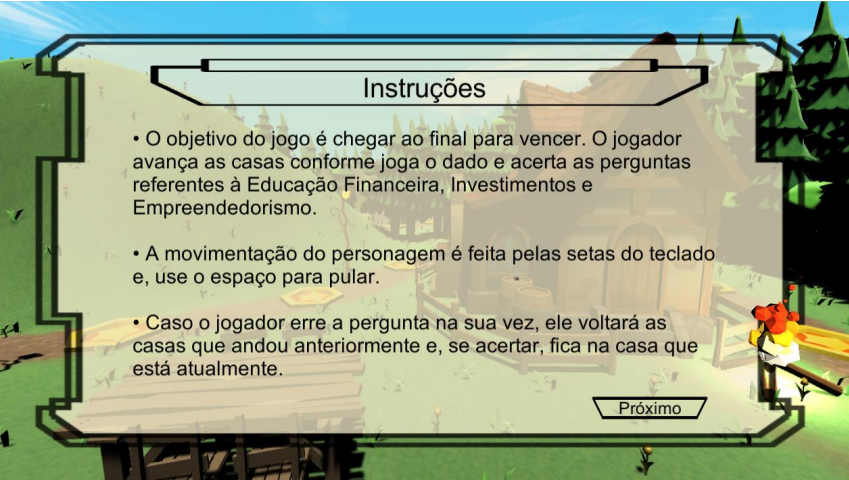
\includegraphics[scale=0.6]{Textuais/Pictures/invest-play-1.png}
	\fonte{\textit{InvestPlay} \cite{santos2020investplay}.}\label{fig:invest-play-1}
\end{figure}

\begin{figure}[ht]
	\centering
	\caption{Cena do jogo \textit{InvestPlay}.}
	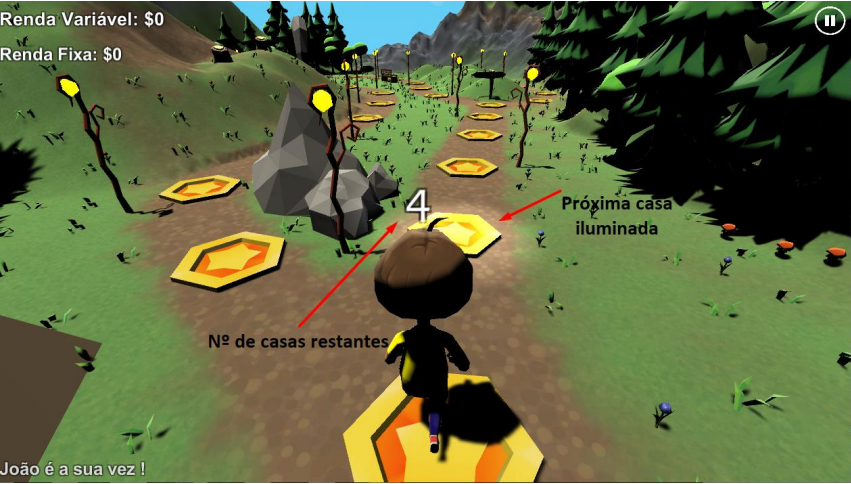
\includegraphics[scale=0.6]{Textuais/Pictures/invest-play-2.png}
	\fonte{\textit{InvestPlay} \cite{santos2020investplay}.}\label{fig:invest-play-2}
\end{figure}

\subsection{Considerações sobre os Trabalhos Correlatos}
Esta seção evidencia a diversidade de abordagens em jogos educativos focados em finanças, cada um com suas características distintas. A gamificação, como demonstrado nos exemplos citados, é uma ferramenta eficaz para a educação financeira, adaptando-se a diferentes públicos e objetivos de aprendizagem. No entanto, ressalta-se a importância de alinhar a metodologia e o conteúdo ao público-alvo, especialmente ao lidar com conceitos financeiros para crianças, onde a simplicidade e a relevância são fundamentais.

\begin{table}[ht]
	\centering
	\renewcommand{\arraystretch}{1.3}
	\caption{Comparativo Aprofundado dos Trabalhos Correlatos}
	\label{tab:comparativo-trabalhos}
	\begin{tabular}{| L{2cm} | L{2cm} | L{2cm} | L{2cm} | L{2cm} | L{2cm} |}
		\hline
		\textbf{}                       & \textbf{Debt Maze}       & \textbf{PlanCash}                    & \textbf{Finance Game}        & \textbf{InvestPlay}               \\
		\hline
		\hline
		\textbf{Público-Alvo}           & Geral                    & Infantil                             & Geral                        & Geral                             \\
		\hline
		\textbf{Metodologia}            & Labirinto                & Jogo de Tabuleiro                    & Simulação                    & Perguntas e Respostas             \\
		\hline
		\textbf{Abordagem Pedagógica}   & Gamificação              & Gamificação e Educação Tradicional   & Simulação Realista           & Dinâmica Interativa               \\
		\hline
		\textbf{Integração Tecnológica} & Média                    & Baixa                                & Média                        & Média                             \\
		\hline
		\textbf{Impacto Educacional}    & Alfabetização Financeira & Conhecimento Financeiro e Matemático & Tomada de Decisão Financeira & Entendimento de Ativos e Passivos \\
		\hline
		\textbf{Baseado na ENEF}        & Não                      & Não                                  & Não                          & Não                               \\
		\hline
	\end{tabular}
	\vspace{2mm}
	\fonte{Elaborado pelo autor (2023).}
\end{table}
